\FloatBarrier
\section[EAMPA]{EAMPA: Potential Analysis and Fitting Code}
\label{code:eampa}

\subsection{Introduction}


A python-fortran based computer code was developed to analyse interatomic potentials and fit their parameters to bulk properties and DFT calculated forces and energies.  It was designed to take advantage of both Fortran and Python.  Fortran is used to compute the neighbour lists, energies, stresses and forces, and Python is used to read and write data, produce plots and control the potential fitting.  This allowed the use of custom optimization subroutines as well as the use of those included in the SciPy module.  Highlights from the code are discussed in this section and the appendix of this work (appendix \ref{chapter:appendix-eampa}).

The latest version of the code has the following features:

\begin{itemize}
\item calculate energy, forces and stress of an ensemble of atoms 
\item calculate bulk properties of a potential for pure \acrshort{bcc} of \acrshort{fcc} structures
\item relaxation of the lattice parameter 
\item relaxation of the cell geometry along with the lattice parameter
\item fitting on analytic potential parameters using simulated annealing, genetic algorithm, Nealder-Meade, Levenberg-Marquardt, BFGS
\item effective gauge transforms of pure element potentials
\item creation of potential files in other formats (tabulated, LAMMPS etc)
\end{itemize}

The source code and instructions on how to use the program are available to download from GitHub.

https://github.com/BenPalmer1983/eampa




%%%%%%%%%%%%%%%%%%%%%%%%%%%%
% Potentials
%%%%%%%%%%%%%%%%%%%%%%%%%%%%

\subsection{Potentials}

The code has been designed specifically for many body potentials.  The function types available for pair, density and embedding are listed in the appendix (\ref{chapter:potentialfunctions}).  More function types may be easily added by editing the module in the Fortran code that defines each function.


%%%%%%%%%%%%%%%%%%%%%%%%%%%%
% Calculations
%%%%%%%%%%%%%%%%%%%%%%%%%%%%



\subsection{Calculations}

The calculations involved in this code centre around the calculation of energy of configurations as well as the forces and stresses when necessary.  All configurations are held within the Python program, but the neighbour list and energy (as well as stress and force) calculations are carried out in an imported Fortran module.

\subsubsection{Energy, Force and Stress Calculations}

A potential and configuration of atoms may be loaded into the program in a number of ways.  Python passes this data to the atom Fortran module and then computes the neighbour list before it is passed back to the Python program where it is stored for later use.

There are a number of functions that allow the potential as well as atom configurations (and neighbour lists) to be updated.  These are handled in Python, but the calculations are carried out in the Fortran atom module, that then passes the results back to Python.  One example of such a function is where the position of the atoms is changed and the neighbour list is updated without a full recalculation.

The energy, forces and stresses may be computed for a range of configurations or a single configuration.  This process starts in Python, but the calculations are once again completed using the Fortran module.  The method used is discussed in section \ref{section:backgroundenergyforcestress} and the subroutine used is included in the appendix (section \ref{section:appendixenergyforcestress}).


\subsubsection{Geometry and Coordinate Optimisation}

Once a configuration is loaded into the program, it can be relaxed using a variety of techniques.  The lattice parameter may be relaxed using the built in \acrshort{bfgs} or \acrshort{cg} minimizers and the same functions may be used to relax the simulation cell.  Where the coordinates of the atoms are relaxed, a damped molecular dynamics subroutine is called from the Fortran module that computes the forces on the atoms and moves them accordingly.  This has been more successful than using built in minimizers, where no gradient data is passed, but a more promising approach might be to include the VA08 subroutine from the Harwell archives\cite{harwellva08}.  This is the same subroutine used in the Bonny potential fitting code\cite{bonnyfecr}.



\subsubsection{Bulk Property Calculations}

The bulk property calculations rely on the calculation of the energy of a number of configurations where specific strains have been applied to the perfect relaxed crystal.  The methods used are discussed in chapter \ref{chap:backgroundfitting} and the subroutine that creates the configurations, with which the module calculates the energies used to plot the equation of state and other distortions, is included in appendix \ref{chapter:appendix-eampa}.

The Python code creates the configurations with the strains applied and the Fortran subroutines are called to compute the energies.  Once the values are collected, the bulk properties are calculated in Python and any required plots are created.

As part of the calculation process the optimum (relaxed) lattice parameter is first calculated for the potential.  Either a \acrshort{bfgs} or \acrshort{cg} minimizer is used.  The basis vectors are fixed by the user, although there could be the option in the future to allow the basis vectors to also be adjusted.  In this work the basis vectors of \acrshort{fcc} \Gls{Fe} were fixed as the tetragonal determined by \acrshort{dft} in the input file for EAMPA.  

During the fitting process, each time the potential is varied, the lattice parameter and bulk properties need to be recalculated.  To save time the neighbour list is only calculated once, and the atom separations are recalculated based on the initial list, the recalculated lattice parameter and basis vectors.


\subsubsection{RSS - How Well The Potential Fits Experimental \& DFT Data}

The fitting process measures how well a potential fits the data when the initial parameters are given and every time a new set of parameters are proposed.  The user assigns weights to configurations and the parameters the potential is being fit to.  The Python code calculates the \acrfull{rss} of the differences between calculated energies, forces, stress, lattice parameter, cohesive energy, bulk modulus and elastic constants and the known values.  The sum of these values measures how well the potential fits.



\subsubsection{Overview of the Potential Fitting Process}

The input files are read in by Python that then iterates over the fitting process while changing the potential.  The Fortran modules calculate the energy, force and stress of the loaded configurations as well as the bulk property calculations for pure crystals of the atomic species and structures specified by the user.  To save on processing time, the neighbour lists for all configurations, including those used to calculate the equation of state and elastic constants, are only calculated once. 

The step by step flow of the program while fitting parameters of a potential is as follows:

\begin{enumerate}
\item Read input files
\item Load Fortran Modules
\item Load potentials into Python
\item Load configurations into Python
\item Create neighbour list configurations in Fortran and save to Python
\item Begin fitting loop in Python
\item Loop starts - loop through potential function parameters
\begin{enumerate}
\item Update potential in Python
\item Create tabulated version of functions
\item Run calculations in Fortran
\item Loop starts - loop through configurations
\begin{enumerate}
\item Calculate energy, force, stress using pre-calculated neighbour lists
\end{enumerate}
\item End loop
\item Save energies, forces and stresses back to Python
\item Compute bulk properties from the energies in Python
\item Calculate the RSS between the potential computed and know values
\item Save parameters if best
\item Make next set of parameters
\end{enumerate}
\item End loop
\item Output results
\end{enumerate}

Once the fitting process has completed, the best set of parameters are stored for the user along with a plot of the potential functions, equation of state and elastic constant energy-strain distortion plots (where these are used in the fitting process).




\subsubsection{Global Optimization}

The EAMPA code has two global optimization algorithms plus a number of other local and global optimization algorithms implemented through SciPy.  These are discussed in greater detail in appendix \ref{chapter:optimization}.

The simulated annealing algorithm is implemented in the code and is an option available to the user for fitting.  The algorithm looks for better solutions and replaces the current value with better values.  It also accepts worse solutions with a probability that decreases with \enquote{temperature}.  

A genetic algorithm has also been implements.  The user chooses the parameters for the algorithm and it attempts to search for the optimum parameters to fit the potential functions to the data.

The user settings include the following:

\begin{itemize}
\item population size
\item \enquote{fresh} (new randomly generated) parameters
\item number of generations
\item how often the best results are enhanced with a chosen local optimization algorithm
\end{itemize}

The function that breeds the parameters randomly combines the parameters from two parent solutions to create two children parameter sets.  The parents are either both from the existing pool of solutions, or a parent from the existing pool with a parent from a fresh set, and the fresh set of parameters changes with each generation (fig. \ref{fig:gabreedevent}).

\begin{figure}[h]
  \begin{center}
    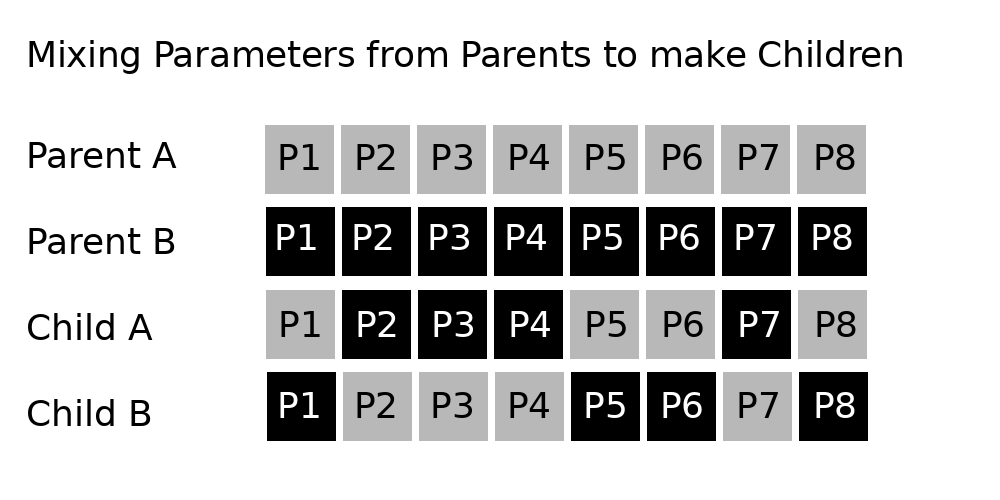
\includegraphics[scale=0.30]{chapters/potentials_fe_pd_ru/images/breeding.png}
    \caption{Parameter Breed Event}
    \label{fig:gabreedevent}
  \end{center}
\end{figure}

There is a chance that the child solutions will mutate slightly from the two parent combination, and there is also a guard that prevents cloning of solutions.  A random selection of the best parameter sets are enhanced periodically using a local optimization method (\acrshort{cg}, \acrshort{bfgs}) and these are introduced to the pool of parameters.



\subsubsection{Minimising Runtime}

When fitting a potential, for each trial set of functions, the program must calculate the energy, forces and stress for each of the configurations and tens or hundreds of energy only calculations for the equation of state and elastic constant calculations.  Python is a well used programming language in many areas of Science and it has the benefits of many modern languages.  For certain specific tasks, it is slow in comparison to Fortran.

The energy, stress and force calculations were programmed in Fortran and use OpenMP to improve the calculation speed.  This could be improved further by processing batches of configurations in parallel, but this isn't currently implemented.  For now, a seed is picked so multiple instances can be run in parallel to give multiple optimised potentials to choose from.

The code optimises analytic potentials, but a number of the functions available are complicated and require the evaluation of many functions in order to give an output.  To speed up the calculation, the user has the option to convert the analytic potentials to tabulated versions and these are interpolated using Lagrange polynomials (eq. \ref{eq:eqLagrangeDataSet} \ref{eq:eqLagrangePolynomialNew}).

\begin{equation}
\begin{split}
D = \lbrace \left(x_0, y_0 \right) \left(x_1, y_1 \right) \left(x_2, y_2 \right) \dotsm \left(x_n, y_n \right) \rbrace
\end{split}
\label{eq:eqLagrangeDataSet}
\end{equation}

\begin{equation}
\begin{split}
p_n (x) = \sum _{i=0} ^n y_i L(i, x) 
\textnormal{where    } l(i, x) = \prod _{j=0 , j!=i} ^n (x - x_j)
\end{split}
\label{eq:eqLagrangePolynomialNew}
\end{equation}

There are typically hundreds or thousands of data points, so to interpolate, the closest few points are used.  The gradient of the potential functions are also computed using Lagrange polynomials (eq. \ref{eq:eqLagrangePolynomialNew}).

%% Sample hybrid function
\begin{equation}
\begin{split}
q_n \left( x \right) = \sum_{i=0}^{i=n} y_{i} g \left(i,  x \right) \\
\textnormal{where    } g \left(i, x \right) = \left( \prod_{j=0, j \neq i}^{j=n} \frac{1}{x_i - x_j} \right) \times \left( \sum_{k=0, k \neq i}^{k=n} \prod_{j=0, j \neq k, j \neq i}^{j=n} \left( x - x_j \right) \right)
\end{split}
\label{eq:eqLagrangePolynomialNew}
\end{equation}

A pseudocode for both interpolation of the function points and derivatives are available in the appendix (section \ref{section:interpolationpseudo} and \ref{section:interpolationgradientpseudo}).



\subsubsection{Effective Gauge Transforms}

In order to create a potential for an alloy an effective gauge transform, as described in section \ref{section:pairembeddingsym}, was applied to each pure potential.  A mode added to the EAMPA program reads in the analytic potential and creates a numeric potential that has had the transform applied.  This allows the pure potentials to be used together, although a cross pair potential is still needed.



\subsubsection{LAMMPS Format}

\acrshort{lammps} is a popular molecular dynamics code and the EAMPA code outputs potentials in its own format as well as the \acrshort{lammps} format.  The structure of the file depends on the number of elements and there are a number of caveats to note including the pair potentials being stored in the file as the value multiplied by the distance, in angstrom\cite{lammpseamformat}.




\subsection{Verifying Energy and Force Calculations with LAMMPS}

Many of the calculations depend on the energies computed as well as accurate computation of the forces.  \acrshort{lammps} is a widely used molecular dynamics code and many potentials already exists in the format required for \acrshort{lammps}.  The energies and forces computed by the EAMPA code were compared for a number of configurations and potentials against the energies and forces computed by \acrshort{lammps} to validate the code developed here.  The results between the two codes agreed.



